\documentclass[sigconf]{acmart}
\usepackage{natbib}
\usepackage{booktabs} % For formal tables
\usepackage{lipsum} % For dummy text
\usepackage{sectsty} % Section header fonts
\usepackage{amsmath}

\AtBeginEnvironment{quote}{\large\bfseries\raggedright\itshape}
\sectionfont{\large\bfseries\raggedright} % Bold, larger, left-aligned
\subsectionfont{\large\bfseries\raggedright} 

\begin{document}

\bibliographystyle{plainnat}
\bibliography{biblio}


\title{MAT 357 Project 2 : "Orbital" Interpolation}
\author{Brillan Morgan}
\author{Osprey Varboncoeur}
\author{Austin Zhu}
\affiliation{%
  \institution{DigiPen Institute of Technology}
  \city{Redmond}
  \state{Washington}
  \country{USA}
}
\email{j.varboncoeur@digipen.edu}
\email{austin.zhu@digipen.edu}
\email{b.preston@digipen.edu}

\begin{abstract}
Your ship is low on fuel, and several belts away from the nearest fueling satellite. Your ship's computer springs to life, stating there may be a slim chance for you to use the Weird gravitational pull of the nearby Hexarian Quantum Giants to slingshot yourself to safety. \\
The only catch, the ship's computer only has enough free processing power to process two constraints at a time, and thus you must use the interpolation theory of control points, with the Quantum Giant's radius as the distance between them to find the an interpolation that will work in this very specific Science Fiction scenario.  \\ \\
This interpolation method hopes to demonstrate a modified version 
\begin{itemize}
    \item Control Points
    \item Radius
    \item Linear Alg + trig 
    \item counter clockwise 
    \item tangent lines at closest intersection
\end{itemize}

\end{abstract}

\keywords{Numerical Analysis, Interpolation, Control Points, Radius, Linear Algebra, Trigonometry}


\maketitle

\section{Problem Statement}

    %\[ \Upsilon(a) = \Gamma(x) - \beta(x) \]
    %\[ \Upsilon(a) = 
    %\begin{cases}
    %    1 & \text{if } \Upsilon(a) > 0 \\
    %    0 & \text{if } \Upsilon(a) < 0
    %\end{cases}
    %\]
  %  \[ \alpha = Action \]
   % Let $\Delta(a)$ \in \mathbb{R}$
   % \[\Delta(a) = \Gamma(x) - \beta(x)
    

\section{Hypothesis}
\begin{quote}
    "There is some $P(x)$ such that \[P(x) \]
\end{quote}
\section{Methodology Analysis}
In the following section we will analyze the proposed solution, highlighting the greatest issues facing its proper implementation. 


\subsection{\textbf{Risks}}
Possible points of failure for a proposed method. 

\subsubsection{\textbf{Risk Case 1}}


\subsubsection{\textbf{Risk Case 2}}
When a curve goes directly from tracing the arc of one circle to tracing the arc of a different circle. That is, there was no distance to trace on a straight line in-between tracing the arcs of the circles. Alternatively, you could think of that line as having zero length. 

(I think) this will happen anytime circle i and circle i+1 are tangent to each other at circle i's radius point. 

If animating a visualization, then changing circle movement/size (also which point is circle i's radius point) could suddenly transition two adjacent circles FROM having a line to trace (of length less than the larger or the two circles' radii) TO having no line to be traced and instead immediately moving on to tracing the arc of circle i+1.


\paragraph{\textbf{Even Weirder: Risk Case 2}}
Possibly even weirder, consider the case where this happens with multiple different circles at the same time? This would mean that (at least) circles i+1 and i+2 are tangent to circle i at circle i's radius point.

How to handle overlapping circles in this context and in general? Do we allow overlapping circles? Maybe we allow overlapping circles, but not adjacent (in i) overlapping circles.

\subsection{\textbf{Mitigations}}
Structural changes made to a methodology in order to provide for goodness

\section{Method Iteration}

\subsection{Math Formulas}

\subsubsection{Linear Algebra}

\subsubsection{Trig}

\subsection{Interpolation Function}


\subsection{Python Stuff\cite{GitHub} }



\section{Interpretation of Point Input Data}
Points in the input set are always interpreted in pairs: center point and radius point, which define a circle. The points in the input data set are numbered 0, 1, 2, ..., n-1, where n-1 is an odd number. Even-numbered point indices correspond to center points of circles. Odd-numbered point indices correspond to radius points of circles.  A valid input data set has an even count of points and represents a total of (n-1)/2 circles.


%% Look above at how to do mathprint

How to interpret input data example:
Three circles (six points) total:
\begin{itemize}
    \item $(x_0, y_0)$ is the center of the first circle
    \item $(x_1, y_1)$ is a point on the edge of the first circle C0, it is the start point of the piecewise curve
    \item $(x_2, y_2)$ is the center of the second circle
    \item $(x_3, y_3)$ is a point on the edge of the second circle C2 through which the piecewise curve must pass
    \item $(x_4, y_4)$ is the center of the third and final circle
    \item $(x_5, y_5)$ is a point on the edge of the third and final circle C4, it is the end point of the piecewise curve
\end{itemize}


\section{Optional Constraints}
Suppose that you wanted to ensure that a curve consisted only of strictly alternating arcs and lines. No adjacent curves from different circles and no No end-to-end lines means we would prohibit input data where any three consecutive circles (in the i sense) are all tangent to the same line

(Do we need to say here that a curve will start with an arc and end with an arc?)
Why might someone want this?
%% TODO: Come up with a rationale for why someone would want this because discussing it gives good content for the paper



What restrictions would you need to place on input data if you wanted to ensure that there were no 


\section{Possible Edge Cases and Cases of Interest}

[For the following items, the expectation is that the items would only be problematic or of note if the property is true for \textit{adjacent} circles (in i) ]
\begin{itemize}
    \item Same circle defined twice.
    \item Two (or more) circles that share the same center, but have different radius points.
    \item A point that is a radius point for two or more different circles.
    \item If any combination of circle center points, radius points or tangent points overlap.
    \item Circles touching in all combinations of ways.
\end{itemize}

The edge of a circle coinciding with the curve at a point where that circle is not "currently" involved in the curve generation ("currently" meaning in terms of what index i "we are at"). Test both with and without that point on the circle "later" becoming involved in the curve generation (implies that the curve went back over itself at that point on the circle).

Test scenarios where computed tangent points are crafted to have integer coordinates which correspond to all combinations of circle center points, radius points or other tangent points. That may not cause any issues, but may be interesting?



Is it problematic/interesting if the two external tangent lines between circle i and circle i+1 parallel? (I'm thinking "no" to both). This would happen with any two adjacent (in terms of i) circles that have the same radius, right?






\begin{verbatim}
LOL, I essentially wrote the same idea twice only a few hours apart ^ v
\end{verbatim}

Prohibit adjacent (in i) circles from overlapping? Though in general, it seems fine for circles to overlap.




\subsection{Data Set Observations (and Observations of Manipulations}

Are there any preconditions or "only in these cases" preface that would make any of these observations (below) more interesting?








\section{Brillan's Development Notes}

\subsection{Figuring Arc Direction}
The arc on circle 0 is a special case in that it is the only circle where the arc STARTS at the radius point and ENDS at the tangent point. For all other circles (i = 2, 4, 6, 8, ...n - 2), the arc STARTS at the tangent point and ENDS at the radius point.
(This is why at first I couldn't get all arcs to look correct at the same time!)



\section{Brillan's P(x) Formula Development Notes}

\subsection{Internal Tangents and Conditionals}
OH, re: Austin’s new version that has internal tangents:
is it the use of internal tangents that makes the conditional for clockwise/counterclockwise necessary?
Can that difference be represented formulaically (mathematically) for the paper?
ChatGPT: “ensure that the theta range calculation correctly accounts for both the start and end angles, especially when the arc crosses the 0 or 360-degree mark.”
Here is my own idea to deal with this if it is not already handled: rotate the circle so that the start/end of the arc is axis-aligned, draw the arc, then rotate the circle back...can do this with matrices, I think.



\subsection{What types of complexity in input data to support?}
Require strictly alternating arcs and lines?
Our code doesn't depend on it, but does our formula?

\subsection{Notes from reading Austin's chatgpt log for getting a P(x) math formula based on the code}
(internal tangents version)

\subsection{Working with t Values}
noting that we have a single t param for the entire curve:
integer part of the t value tells you which arc or line function to call
fractional part of the t value tells you what value to pass to the arc or line function: 0 to 1 for each piece of the curve.
Beginning of curve is in arc $A_0$ at t = 0 (pass 
The very end point of the curve is plotted as a single 

From reading Austin's chatgpt log: it doesn't include HOW to determine what the specific line segments and arcs are, only how to express them once you know what they are

from where i'm reading now, requiring that no adjacent circles intersect would simplify the logic by removing a conditional
(adjacent in terms of position in the input data, i, not geometrically adjacent)...but i think you still need conditionals even with external tangents only

\begin{figure}
    \centering
    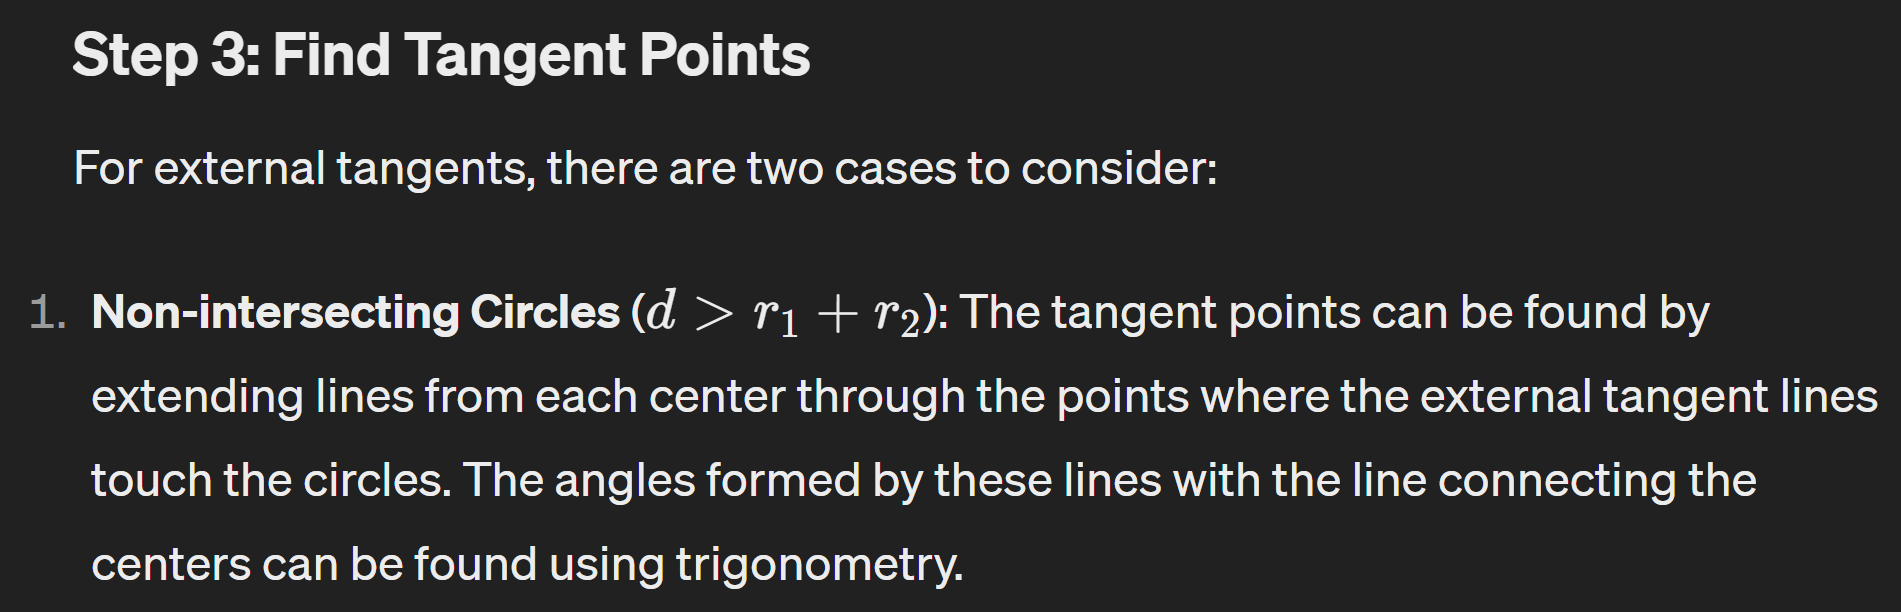
\includegraphics[width=0.5\linewidth]{Non-IntersectingCircles_FindTangentPoints.png}
    
    
\end{figure}
\begin{figure}
    \centering
    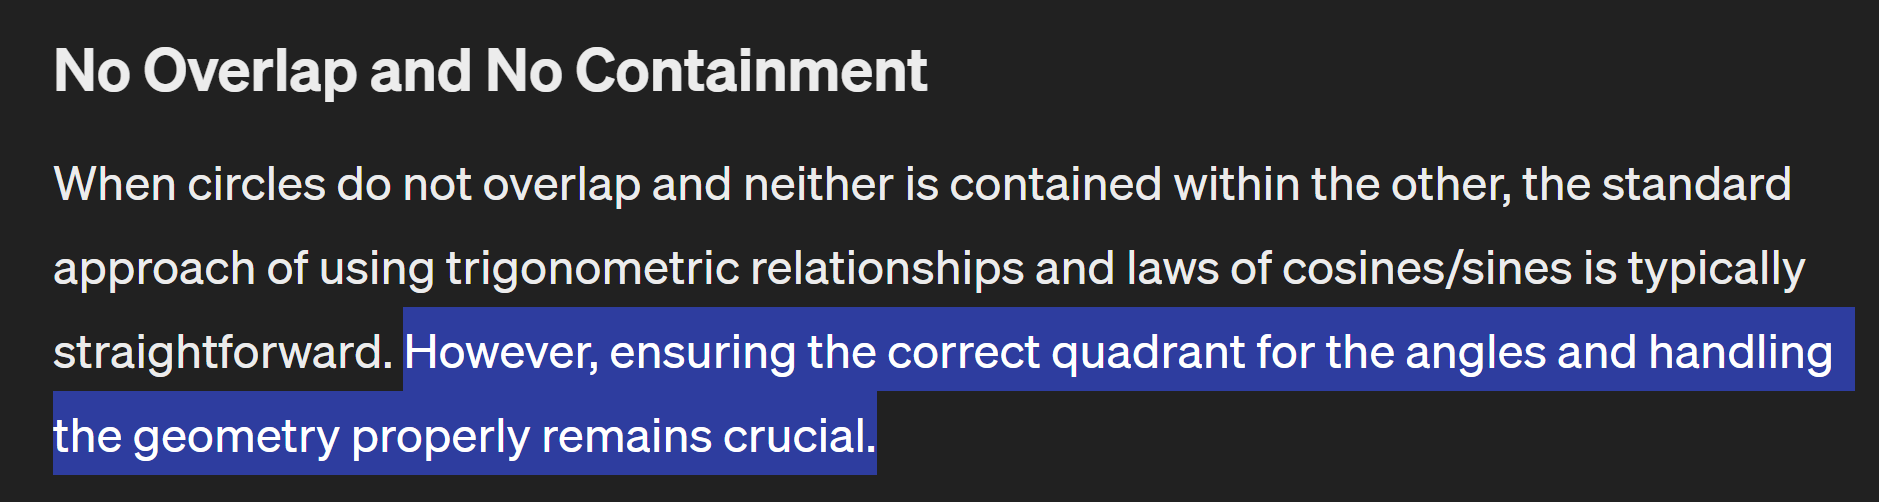
\includegraphics[width=0.5\linewidth]{NoOverlapNoContainment_FindTangents.png}
    
    
\end{figure}

in the basic version of the math expression...do we need to be concerned with "\textbf{ensuring the correct quadrant for the angles} and handling the geometry properly?"





\section{Animation Ideas}
Cool ways that we can animate our results?
Rendering of an (unchanging) curve. At a constant speed? Slower on arcs, faster on lines?
Circles getting larger/smaller. (radius changes, so adjust radius point in/out proportionally)
Circles moving
Radius point moving along the edge of its circle (radius not changing)

Any of the above animations happening in response to the animation of the curve render approaching toward (or departing from) that circle/point that is on the curve.

Create sliders or some other way to control some parameters of the curve interactively.

Could animate the rendering of the curve while on an arc by which "arc departure" prerequisites are currently being met: neither, radius point traced, 


\subsection{PYTHON REPO LINK}
\href{https://github.com/BrillanShare/mat357-557-project-2}{https://github.com/BrillanShare/mat357-557-project-2}



\section{Walking Through How Austin's Code Version Works in English}

For brevity and to disambiguate, lines marked with (A) are direct observations about what Austin's code does
Other lines are my commentary, suggestions, intentions
%(^ but I stopped doing this after a while, whoops)

\subsection{Starting Arc Direction[}
(A) Starting arc direction for the first circle is set to counterclockwise (arbitrarily)
What is easier/better for our math expression? Currently, I have my desmos plot going from the anchor point to the tangent point that is the furthest away. That is, the tangent point which would create the longest arc.

\subsection{Reversed Meanings of "Anchor" and "Control" Points}
(A) The circle center points are referred to as "Control" points and the circle edge points are referred to as "Anchor" points.
These meanings of "Anchor" and "Control" points are backwards from my desmos plot and everything I've written here in this doc and on paper.

\subsection{Indexing of Arc and Line Functions Based on Usage of Fractional t Values}
(A) Anchor and Control functions provide 1-based lookup of the ith Anchor point, and Control point, respectively. (Remember that the meanings of each are reversed in Austin's code)

For our math expression, because of how our piecewise function works with t - $\lfloor$ t $\rfloor$ , it will be way easier to have the Arc functions at even indices starting at zero: 0,2,4... and the Line functions at odd indices starting at one: 1,3,5... That way, the alternating Arc and Line function indicies will increase by one at each step. Specifically, it will make it cleaner for each line to refer to the arc before it (index - 1) and the arc after it (index + 1). Similarly, each arc can refer to the line before it (if it exists) with index - 1 and the line after it (if it exists) with index + 1.

Furthermore, with this indexing scheme, every time we go 0 <= t - $\lfloor$ t $\rfloor$ < 1, that will correspond to either a specific arc or a specific line, rather than the composite of an arc with the line that follows it. The meaning of a fractional t value is much clearer when 0 <= t - $\lfloor$ t $\rfloor$ < 1 corresponds to a single geometric object, rather than a composite one.

In contrast, if 0 <= t - $\lfloor$ t $\rfloor$ < 1 corresponded to an arc with the line that follows it, it would not be immediately obvious how much of that t value would belong to the arc and how much would belong to the line. Furthermore, it would not be clear whether that proportion would be consistent across different arc/line pairs.

Better to have 0 <= t - $\lfloor$ t $\rfloor$ < 1, correspond to either a specific arc or a specific line. (mic dr4op)

\subsection{Proposed Code Revisions So Far}
So far, the revisions I've proposed to Austin's code are:
Make "Anchor" correspond to circle center points and "Control" correspond to circle edge points.
...hrm, maybe the lookups for Anchor and Control just need to be changed to be zero-based. Then you could interpret them just as corresponding to their indexed circle. That is, not corresponding directly to Arc function or Line function referenced in our math expression.

\subsection{What to show in plot_debug}
(A) Currently with the plot debug setting off, a bunch of extra things are plotted in addition to the output curve
With plot debug off, I think we should only plot the output curve
Then with plot debug on, show all the extra visual info


\subsection{Primary for loop iterates over i from 1 to n/2}
Where n is the total number of points and n/2 is the number of circles.

So, for every pair of circles
First iteration is: circle1 and with center1, edge1 and circle2 with center2, edge2

Now lining the python code up with what I've got in desmos:

Get external tangents:

    Circle radii:
    r1 for circle1, r2 for circle2
    
    Get distance between the centers of the two circles:
    d in python, d1 for the first pair in desmos

    Get the angle of the line connecting the centers of the circles
    called theta in python, computed with arctan2 (to respect which quadrant the angle is in)
    called alpha in desmos. I tried to use arctan2 in desmos in a bunch of different ways, but could never get it to work. eventually relented: could only get the right answer in desmos with regular arctan. this will cause division by zero if the circles have the same x coordinate (if they are vertically stacked), and potentially (but not for certain?) cause issues because of the quadrant concern). \textbf{i don't know why arctan2 doesn't give the expected result in desmos.}

    (Only looking at external tangents rn, skipping over internal tangent code)
    (Looks like I got lucky that my hand-drawn example wouldn't involve internal tangents according to Austin's code)

    Given that one circle is not inside the other, abs(r1 - r2) > d, external tangents will exist.
    
    Get the angle of the line connecting the centers of the circles
    called phi in python
    called theta in desmos
    calculated the same way

    In python, Austin makes an array angles where
    angles[0] is the sum of the angles: theta + phi in python, alpha + theta in desmos
    angles[1] is the difference of the angles: theta - phi in python, alpha - theta in desmos

    Given the pattern in how these angle combinations are used, I think it would be clearer to visually retain the +, - instead of reducing it to angles[0] and angles[1]

    Perhaps most importantly, ideally would make sure that for the pair of circles starting with circle i, that the tangents (array of tangent points) be organized as TiA, TiB, TiC, TiD
    That is, use the (+) sum of angles first (for TiA, TiB)
    and use the (-) difference of angles second (for TiC, TiD)

    Also, within the two +/- cases above,
    Use the center point of circle1 first (for TiA/TiC), then use the center point for circle2 second (for TiB/TiD)

    Ok, let's see what order Austin did them in:
    Sums first, good
    Circle1 first, good

    Excellent, the tangent points should be organized as reflected in my drawing and in desmos:
    TiA, TiB, TiC, TiD (for tangent points of tangent lines of circle i extending to circle i+1)

    Oh, actually Austin is organizing them like this...which seems fine:
    %tangents[0] = {TiA, TiB} # external tangent points on one side or the circles (that is, both on the same line)
    %tangents[1] = {TiC, TiD} # external tangent points on the other side of the circles (both on the other line)
    
    ...though ideally we would update naming and numbering to be as similar as reasonable between the python and desmos

    Debug plotting of all tangent lines in blue dashes (ahead of determining which tangent line the curve path will take from circle i to circle i+1

    Now "find the tangent point in the corresponding direction"
    Noting that the "clockwise" variable is global and starts arbitrarily as false for the first circle
    c = 0 if clockwise
    c = 1 if counterclockwise
    ...this is confusing...why not just use the clockwise variable directly?
    also why have clockwise == True correspond to c == 0 and clockwise == False correspond to c = 1?

    Is this meaning to indicate a change of direction at this point? If so, why not indicate that?

    For find arc degree...
    
    
    




\end{document}
